The result obtained in our face recognition system with DB1 is dependent on the images being taken in an environment with no distracting background. With this problem in mind there were problems getting any okay result at all on DB2, the database containing the challenging images of persons in the reference database. What happened was that the cluttered background contains skin-like parts that confuse the facial feature detection algorithm, and makes it think that there is skin where there is none. This leads to a situation where the skin detection, whose main purpose is to aid the eye and mouth detection, returns an unreasonably large mask. Within this large mask, there might be several eye and mouth candidates, which combined together creates faulty face candidates. An improvement of the implementation discussed in this paper could therefore be some better face detection method to easier mask out the areas with disturbance.

As can be seen in table 3, some images did not respond to the countermeasures taken against the distortion that the images were exposed to. Image number 9 only had one correct match out of 27, and in image number 7 there were 9 attempts where no face was found and the program canceled before any matching attempt were made. To understand what is going on in these particular cases, we take a look at the process of the face detection and normalization.

In the images in figure \ref{fig:darkrotscal} to \ref{fig:mouth7}, the face detection process of image 7 is shown, where the image is darkened, rotated and scaled. As can be seen in figure \ref{fig:darkrotscal}, the face mask that is the result of the skin model function only returns a very small part of the whole face. This is the source of the issue – no face is detected since the eyes are excluded by the face mask. This is likely due to the lowered tone value of the image. 

\begin{Figure}
  % center it!
  \centering
    % adjust width as you like, include image from optional folder
    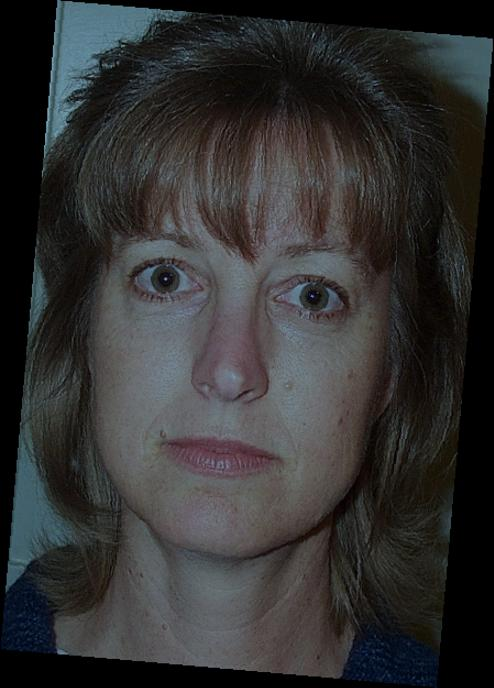
\includegraphics[width=0.5\columnwidth]{im7_img.jpg}
    % caption! change the label ref to what you want
    \captionof{figure}{\emph{Image darkened, rotated and scaled}\label{fig:darkrotscal}}
\end{Figure}

\begin{Figure}
  % center it!
  \centering
    % adjust width as you like, include image from optional folder
    
\includegraphics[width=0.5\columnwidth]{im7_mask.jpg}
    % caption! change the label ref to what you want
    \captionof{figure}{\emph{Image masked}\label{fig:mask7}}
\end{Figure}

\begin{Figure}
  % center it!
  \centering
    % adjust width as you like, include image from optional folder
    
\includegraphics[width=0.5\columnwidth]{im7_eye.jpg}
    % caption! change the label ref to what you want
    \captionof{figure}{\emph{Eye map of image}\label{fig:eye7}}
\end{Figure}

\begin{Figure}
  % center it!
  \centering
    % adjust width as you like, include image from optional folder
    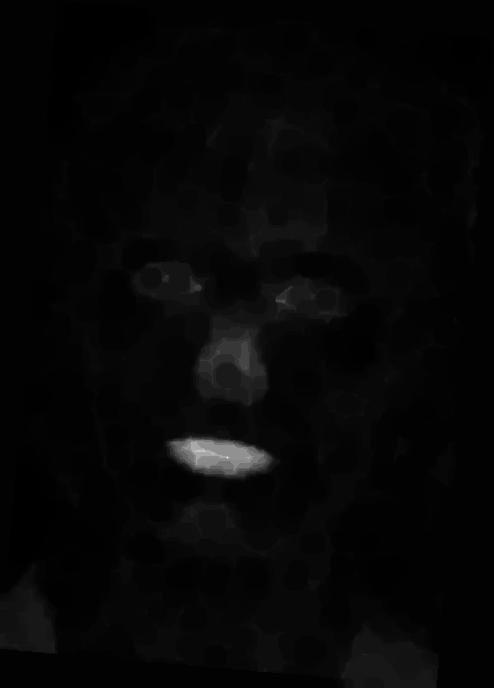
\includegraphics[width=0.5\columnwidth]{im7_mouth.jpg}
    % caption! change the label ref to what you want
    \captionof{figure}{\emph{Mouth map of image}\label{fig:mouth7}}
\end{Figure}


In the images in figure \ref{fig:darkrotscal9} to \ref{fig:normalized9}, we see the completed detection and normalization of a rotated, lightened and scaled version of image 9. The normalization and facial detection works fine on this example, however it was registered as a false positive. The system guessed that this was a picture of another person. 


\begin{Figure}
  % center it!
  \centering
    % adjust width as you like, include image from optional folder
    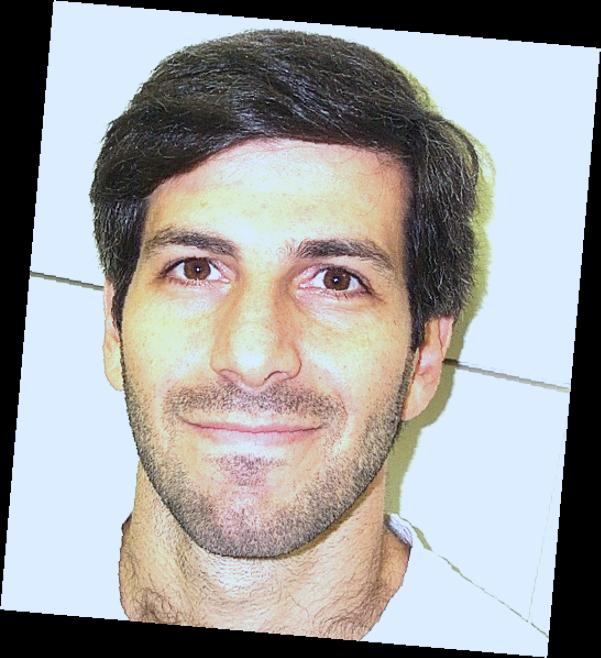
\includegraphics[width=0.5\columnwidth]{im9_img.jpg}
    % caption! change the label ref to what you want
    \captionof{figure}{\emph{Image darkened, rotated and scaled}\label{fig:darkrotscal9}}
\end{Figure}

\begin{Figure}
  % center it!
  \centering
    % adjust width as you like, include image from optional folder
    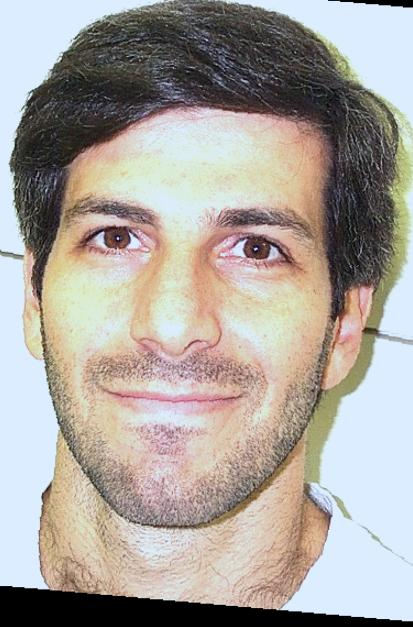
\includegraphics[width=0.5\columnwidth]{im9_cropped.jpg}
    % caption! change the label ref to what you want
    \captionof{figure}{\emph{Image cropped}\label{fig:crop9}}
\end{Figure}

\begin{Figure}
  % center it!
  \centering
    % adjust width as you like, include image from optional folder
    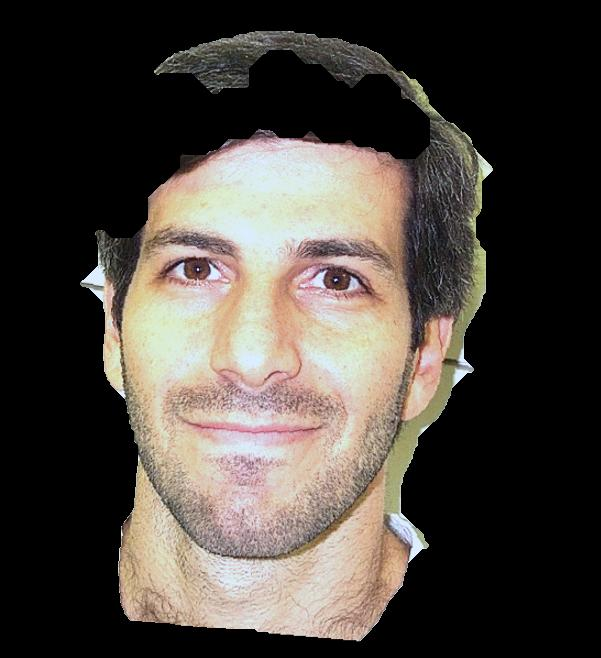
\includegraphics[width=0.5\columnwidth]{im9_mask.jpg}
    % caption! change the label ref to what you want
    \captionof{figure}{\emph{Image masked}\label{fig:mask9}}
\end{Figure}

\begin{Figure}
  % center it!
  \centering
    % adjust width as you like, include image from optional folder
    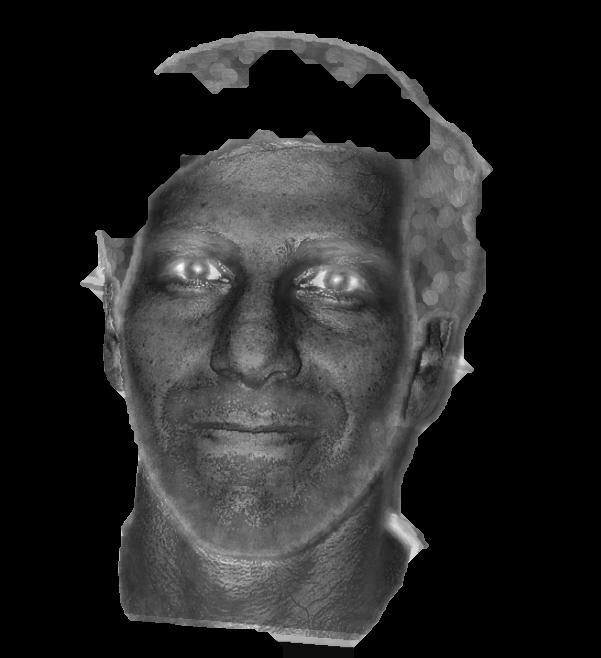
\includegraphics[width=0.5\columnwidth]{im9_eye.jpg}
    % caption! change the label ref to what you want
    \captionof{figure}{\emph{Eye map of image}\label{fig:eye9}}
\end{Figure}

\begin{Figure}
  % center it!
  \centering
    % adjust width as you like, include image from optional folder
    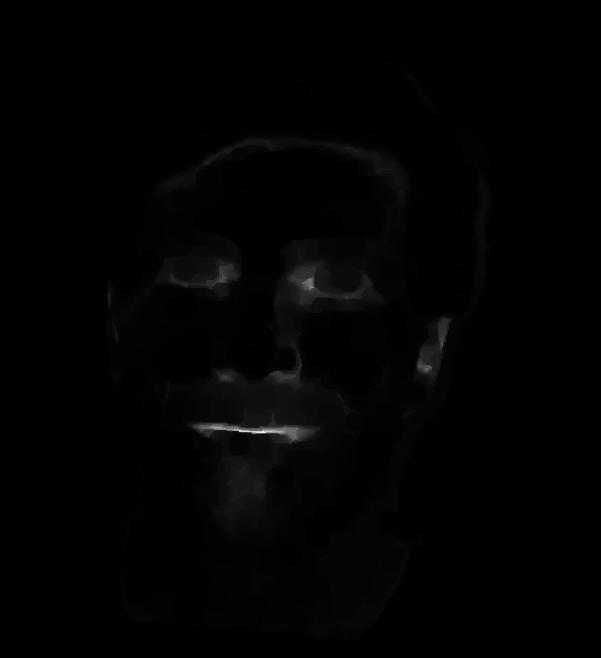
\includegraphics[width=0.5\columnwidth]{im9_mouth.jpg}
    % caption! change the label ref to what you want
    \captionof{figure}{\emph{Mouth map of image}\label{fig:mouth9}}
\end{Figure}

\begin{Figure}
  % center it!
  \centering
    % adjust width as you like, include image from optional folder
    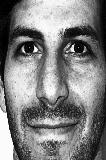
\includegraphics[width=0.5\columnwidth]{im9_normalized.jpg}
    % caption! change the label ref to what you want
    \captionof{figure}{\emph{Image normalized}\label{fig:normalized9}}
\end{Figure}


\subsection{Fisherfaces}
One method that could have been used instead of Eigenfaces to increase the success of our recognition is Fisherfaces. FIsherfaces rely on linear discriminant analysis (LDA), a method that succeed Fisher's linear discriminant method (hence the name Fisherfaces) and that recognises patterns in a set of images. Similar to PCA, this method focus a lot on dimensionality reduction. This method would replace the Eigenfaces state, where the faces are recognised and not detected, of the system discussed here.

However, Fisherfaces is a method that greatly benefits from having several photos of the same class, in our case image of a face. Here, Fisherfaces focuses on maximizing the ratio of the between-class differences and the within-class differences (Eigenfaces vs. Fisherfaces: Recognition using class specific linear projection). Since we do know which class, again; face, each image belong to, we can use images from DB2 to create a better performing Fisherface database. This method can be considered more complex than Eigenfaces and relies on a solid and reliable facial detection system. Also, before this could be implemented, an improved face detection that works well on DB2 would have to be implemented.

According to Eigenfaces vs. Fisherfaces: Recognition using class specific linear projection, Eigenfaces has a higher error-rate when parameters such as lightning and expression vary. Therefore, the system is likely to benefit from an implementation of Fisherfaces. Other than the increased complexity, there isn’t really anything negative with Fisherfaces compared to Eigenfaces.


\subsection{LogAbout}
LogAbout was implemented and is available as an extra normalization feature in the program. However it was hard to find values that performed well for the given datasets. The problem that was  found was that it was hard to determine what values the constants a, b, and c should have in the equation. In the researched papers for the implementation of LogAbout there were no given constants since every dataset has its own values that fit for it.  Therefore attempts were made to determine the constants by trial and error. There were no good results that came out of this and it was settled that the LogAbout method were not to be used in our implementation since it only worsened the final result.
